% DRAFT. Simulation results are measured (data/sweep.csv). Everything marked TODO needs the team.
\documentclass[conference]{IEEEtran}
\usepackage{amsmath,amssymb,graphicx,booktabs,xcolor}
\newcommand{\todo}[1]{\textcolor{red}{[TODO: #1]}}
\newcommand{\qd}{\dot{q}}
\begin{document}
\title{Reactionless Compliance: Which Redundancy Resolution Should a Teleoperated Free-Floating Servicer Use?}
\author{\IEEEauthorblockN{\todo{five names}}\IEEEauthorblockA{MA6223 Human--Robot Interaction, Nanyang Technological University}}
\maketitle

\begin{abstract}
A robot arm on a free-floating spacecraft pushes its own base around whenever it moves. A 7-joint
arm has spare freedom that can be spent on cancelling that push, on keeping the arm's shape
predictable for the operator, or on neither. We compare five redundancy resolution schemes in a
momentum-conserving MuJoCo simulation, on three servicer sizes (30, 300 and 3000\,kg base, 12.5\,kg
arm) and two task types (position only, and position plus orientation). With a position-only task
the reactionless schemes cut peak base attitude drift by a factor of six on the 300\,kg servicer
(0.20$^\circ$ against 1.22$^\circ$) with tracking still under 0.2\,mm. With a full 6-D task the freedoms run
out, and drift can only be bought with tracking error: on the 30\,kg servicer, staying inside a
5$^\circ$ pointing limit costs about 80\,mm of hand error. On the 3000\,kg servicer the choice of scheme
changes base drift by less than 0.01$^\circ$, so the spare freedom is better spent on the operator.
A contact-speed map from ISO/TS 15066 gives 0.28 to 0.76\,m/s depending on servicer size and
posture. A participant study of operator predictability is specified but not yet run.
\end{abstract}

\section{Introduction}
On-orbit servicing puts a human operator in control of an arm whose base is not bolted down.
Momentum is conserved, so every hand motion rotates the spacecraft, which moves antennas and
sensors off their targets~\cite{dubowsky1993,umetani1989}. Reaction null-space (RNS) control uses
arm redundancy to move the hand without rotating the base~\cite{nenchev1999,yoshida2001}.
Separately, human--robot interaction work shows that operators do better when the arm's
configuration is repeatable, which null-space impedance toward a rest posture
provides~\cite{hogan1985,dragan2013}. Both draw on the same small pool of spare joints.

\textbf{Gap.} Reactionless control is studied for what it does to the spacecraft, and null-space
compliance for what it does to the person. We found no study that puts both on the same arm and
asks what the operator gives up for a quiet base, or how the answer changes with spacecraft size.

\textbf{Contributions.} (i) A degree-of-freedom argument, checked numerically, for when a quiet
base is free and when it is not. (ii) A five-scheme, three-size, two-task benchmark with a
verified momentum-conserving model. (iii) The trade-off curve between hand error and base drift.
(iv) A contact-speed map per servicer size. (v) A ready-to-run protocol for the operator study.

\section{Related Work}
\todo{P2: condense P2\_Literature\_Survey.xlsx to about half a page.}
The generalised Jacobian~\cite{umetani1989} gives hand motion of a free-floating arm from joint
rates alone. RNS~\cite{nenchev1999} and its flight test on ETS-VII~\cite{yoshida2001} show
zero-reaction manoeuvres. Damped least squares~\cite{nakamura1986} and gradient
projection~\cite{liegeois1977} are the standard redundancy baselines. Effective mass at the
contact point~\cite{khatib1995} links arm posture to collision severity, the basis of the
power-and-force limiting mode in ISO/TS 15066~\cite{iso15066,haddadin2012}.

\section{Model}
The system is a rigid base on a free joint with a 7-revolute arm (z-y-z-y-z-y-z, reach 1.09\,m),
no gravity, simulated in MuJoCo~\cite{todorov2012} at 0.5\,ms with RK4. With base twist $v_b$ and
joint rates $\qd$ the mass matrix splits as
\begin{equation}
M=\begin{bmatrix}H_b & H_{bm}\\ H_{bm}^{\!\top} & H_m\end{bmatrix},\qquad
H_b v_b + H_{bm}\qd = 0
\end{equation}
when starting from rest. So $v_b = V\qd$ with $V=-H_b^{-1}H_{bm}$, and the hand twist is
\begin{equation}
\dot{x} = (J_m + J_b V)\,\qd = J^{*}\qd .
\end{equation}
Let $W$ be the three angular rows of $V$. The base does not rotate exactly when $W\qd=0$.
(Using the null space of the angular block of $H_{bm}$ instead is only correct when the base frame
is at the system centre of mass.)

\textbf{Verification.} Under random joint commands for 10\,s the base-row momentum stays below
$10^{-6}$ in SI units on all three servicers, and $J^{*}\qd$ and $W\qd$ match the simulated hand
and base velocities to $10^{-6}$.

\textbf{Freedom count.} $W$ has rank 3, leaving a 4-dimensional reactionless subspace. A
position-only task needs 3, so $3+3=6\le7$: exact, with one joint to spare. A 6-D task needs
$6+3=9>7$: no exact solution exists. Both statements are checked by rank tests on all sizes.

\section{Schemes}
All schemes output joint rates, tracked by joint velocity servos and limited to 2\,rad/s by
scaling the whole vector. $q_0=-k_p(q-q_{\mathrm{rest}})$.
\begin{enumerate}
\item \textbf{DLS}: $\qd=J^{*\top}(J^{*}J^{*\top}+\lambda^2I)^{-1}\dot{x}$.
\item \textbf{Gradient projection}: pseudo-inverse plus manipulability gradient in the null space.
\item \textbf{Null-space impedance}: pseudo-inverse plus $q_0$ in the null space.
\item \textbf{RNS}: task and $W\qd=-k_a\,\theta_b$ together, $\theta_b$ the base attitude error.
\item \textbf{Impedance + RNS}: as 4, with $q_0$ in whatever freedom is left.
\end{enumerate}
For the position-only task, 4 and 5 stack $[J^{*}_{pos};W]$ and solve exactly. For the 6-D task
they solve
\begin{equation}
\qd=(J^{*\top}J^{*}+\beta W^{\top}W+\gamma I)^{-1}(J^{*\top}\dot{x}-\beta k_a W^{\top}\theta_b+\gamma q_0),
\end{equation}
where $\beta$ sets how much hand accuracy is traded for a quiet base.

\textbf{Joint limits.} Every scheme is wrapped in the same guard. A joint within 0.05\,rad of its
limit ($\pm2.9$\,rad on the roll joints, $\pm2.0$\,rad on the pitch joints) that is still commanded
outward is locked, and the remaining joints re-solve. The hand task is weighted above the
reactionless term, so whatever the locked joints can no longer cancel goes into base motion
rather than hand error. In the scripted benchmark only pure RNS reaches a limit (36\% of the run
on the 300\,kg servicer); no run exceeds one.

\section{Experiment}
The hand follows a 0.10\,m circle in the x-z plane of the inertial frame, twice, 15\,s per loop, starting and
ending at rest; the 6-D task adds a 0.25\,rad tool tilt. A scripted operator (feed-forward plus
proportional correction) stands in for the human so that runs are repeatable. Design: 5 schemes
$\times$ 2 tasks $\times$ 3 sizes, plus $\beta\in[10^{-2},10^{6}]$ for schemes 4 and 5 in 6-D.
Measures: RMS hand position error, peak base attitude drift, joint return error
$\|q_{\mathrm{end}}-q_{\mathrm{rest}}\|$, smallest singular value of $J^{*}$. All 84 runs were stable.

\section{Results}
\begin{table}[t]
\caption{Position-only task: hand error / peak base drift}\label{tab:3d}
\centering\begin{tabular}{lccc}\toprule
Scheme & 30\,kg & 300\,kg & 3000\,kg\\\midrule
DLS & 0.14\,mm / 17.9$^\circ$ & 0.12 / 1.22 & 0.12 / 0.040\\
Grad. proj. & 0.08 / 16.4 & 0.11 / 1.08 & 0.12 / 0.037\\
Impedance & 0.08 / 19.7 & 0.11 / 1.23 & 0.12 / 0.040\\
RNS & 47.0 / 3.97 & 0.16 / 0.22 & 0.10 / 0.016\\
Imp.+RNS & 49.7 / 1.94 & 0.16 / 0.20 & 0.11 / 0.027\\\bottomrule
\end{tabular}\end{table}

\textbf{Position-only task (Table~\ref{tab:3d}).} On the 300\,kg servicer the reactionless schemes
cut peak drift five to sixfold with tracking still under 0.2\,mm. With scheme 5 the base returns to its start
attitude (0.01$^\circ$). Plain RNS ends 0.13$^\circ$ off because one joint drifts onto its limit, and the others end 0.4 to 0.7$^\circ$ off. Drift is not exactly
zero as the freedom count predicts; we attribute the remainder to velocity-servo lag, which the
attitude feedback corrects only after it appears. \todo{confirm by rerunning with ideal joint
rates.} On the 30\,kg servicer the reactionless solution holds a joint on its limit for 24 to 44\% of the run,
so the hand falls 47 to 50\,mm behind and the base still turns 2 to 4$^\circ$: a quiet base is feasible in principle and not on this path.

\begin{figure}[t]\centering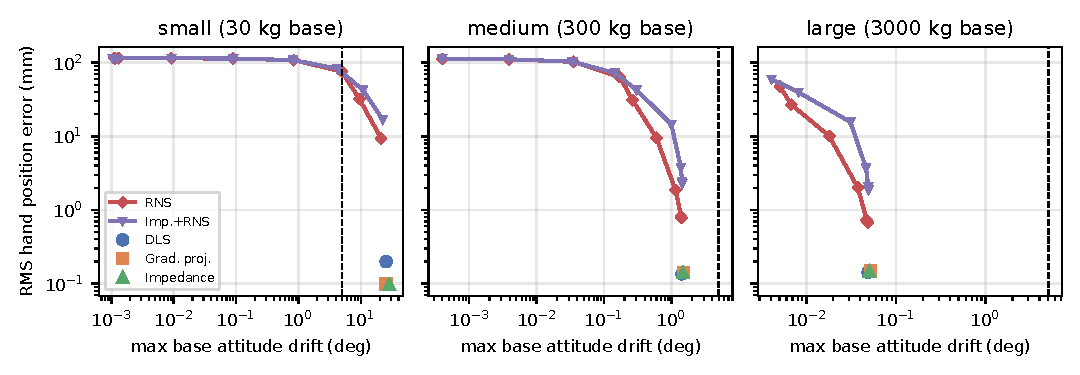
\includegraphics[width=\columnwidth]{figs/fig1_tradeoff}
\caption{6-D task. Each line is one reactionless scheme as $\beta$ goes from $10^{-2}$ to $10^{6}$.
Dashed: 5$^\circ$ pointing limit.}\label{fig:trade}\end{figure}

\textbf{6-D task (Fig.~\ref{fig:trade}).} There is no free lunch. On the 300\,kg servicer RNS moves
from 1.7\,mm error and 1.5$^\circ$ drift ($\beta=10^{-2}$) to 56\,mm and 0.32$^\circ$
($\beta=10^{2}$), and at $\beta=10^{6}$ the base is still and the hand barely follows (114\,mm).
On the 30\,kg servicer schemes 1 to 3 drift 45 to 48$^\circ$, far outside a 5$^\circ$ limit; getting
inside it needs $\beta\ge1$ and costs 81 to 84\,mm.

\begin{figure}[t]\centering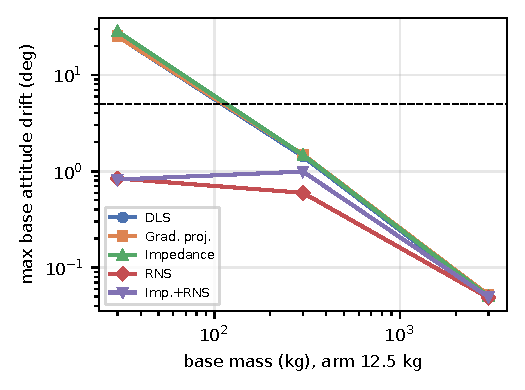
\includegraphics[width=.9\columnwidth]{figs/fig2_size}
\caption{Peak base drift against base mass, 6-D task, $\beta=10$.}\label{fig:size}\end{figure}

\textbf{Servicer size (Fig.~\ref{fig:size}).} Drift falls about 30 times for each tenfold step in base mass. At
3000\,kg every scheme stays under 0.05$^\circ$ and the reactionless term buys nothing measurable
in 6-D, while costing 1.3 to 3.7\,mm of tracking.

\begin{figure}[t]\centering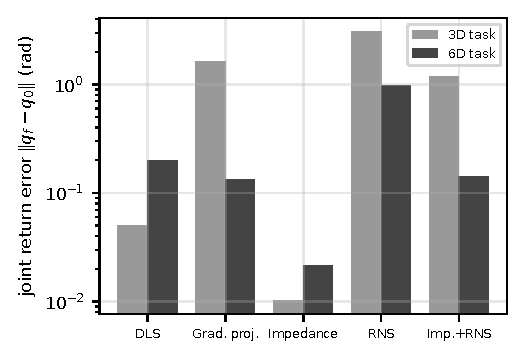
\includegraphics[width=.9\columnwidth]{figs/fig3_jointdrift}
\caption{Joint return error after two loops, 300\,kg servicer.}\label{fig:drift}\end{figure}

\textbf{Joint drift (Fig.~\ref{fig:drift}).} Null-space impedance returns the arm to its rest shape
(0.010\,rad position-only, 0.021\,rad 6-D); DLS ends 0.05 to 0.20\,rad away. Pure RNS is the worst
by far (3.1\,rad position-only, on a joint limit for half the run), because it spends all spare freedom on the base. Adding impedance
to RNS recovers part of that position-only (1.18\,rad) and most of it in 6-D (0.14 against 0.97\,rad), with
slightly less base drift in the position-only task (0.20 against 0.22$^\circ$).

\begin{table}[t]
\caption{Straight-line hand reach from rest against base drift allowed (hand first, $w=2$)}\label{tab:reach}
\centering\begin{tabular}{lccc}
\hline
Drift allowed & 30\,kg & 300\,kg & 3000\,kg\\
\hline
0.5$^\circ$ & 0.15 & 0.25 (0.11--0.37) & 0.61\\
1$^\circ$ & -- & 0.31 (0.17--0.48) & --\\
2$^\circ$ & 0.18 & 0.46 (0.27--0.70) & 0.61\\
none & -- & 0.59 (0.27--1.20) & --\\
\hline
\multicolumn{4}{l}{\footnotesize Mean over $\pm x,\pm y,\pm z$ in metres (range); arrival within 5\,mm.}
\end{tabular}\end{table}

\textbf{What a level base costs in reach (Table~\ref{tab:reach}).} Restricted to the joint motions
that do not turn the base, the hand Jacobian of the 300\,kg servicer at rest has singular values
0.36, 0.10 and 0.08, against 0.22 to 0.74 unrestricted: one direction stays about four times freer
than the other two. Over 6000 random postures the smallest value has median 0.01 and
never exceeds 0.10, so no starting posture removes the limit, and from 0.08 at rest it falls to 0.007
after 0.15\,m forward and below 0.0001 after 0.14\,m sideways, a dynamic singularity \cite{dubowsky1993}. Reach is therefore bought with drift. The
price is set by base inertia: at rest the worst hand direction turns the base by 9.9$^\circ$,
0.76$^\circ$ and 0.03$^\circ$ per 10\,cm on the 30, 300 and 3000\,kg servicers. Holding the hand still leaves the spare joints 10 to 20\% of their authority
over the base, so the base only partly re-levels at the goal
(1.52$^\circ$ on arrival, 0.79$^\circ$ after 8\,s, one joint on its limit). The drift does not fully come back
with the hand either. From the earlier rest pose it did (0.00$^\circ$ after 0.3\,m out and back). From the ready
pose 0.30$^\circ$ is left, with the joints 1.24\,rad from where they started, and three laps of a square leave
0.67, 0.11 and 0.14$^\circ$. Base tilt is only roughly a function of where the hand is.

\begin{figure}[t]\centering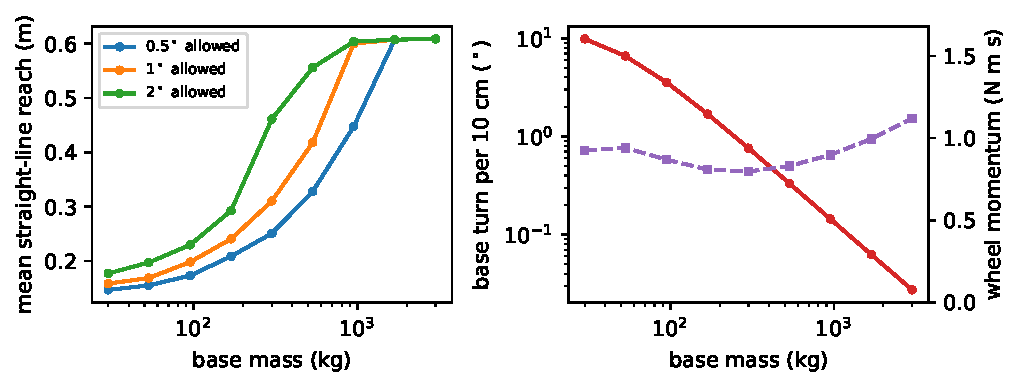
\includegraphics[width=\columnwidth]{figs/fig6_sizing}
\caption{Left: mean straight-line reach against base mass for three drift limits. Right: base turn per 10\,cm of hand
travel (solid) and the momentum reaction wheels would carry to cancel it at 0.1\,m/s (dashed).}\label{fig:sizing}\end{figure}

\textbf{Sizing (Fig.~\ref{fig:sizing}).} Nine base masses from 30 to 3000\,kg give a design chart for this 12.5\,kg arm:
the full 0.61\,m straight-line reach needs about 1700\,kg at a 0.5$^\circ$ limit and about 950\,kg at 2$^\circ$; a
100\,kg servicer keeps 0.17 to 0.23\,m. Holding the base with reaction wheels instead does not get cheaper on a
bigger bus: the momentum they must carry is $h=Kv$ for hand speed $v$, with $K$ between 8 and 11\,kg\,m at rest across
all nine masses (median 8, 90th percentile 13 over 2000 postures at 300\,kg), because it is the arm's momentum and
not the base's. At the 0.1\,m/s used here that is 0.8 to 1.1\,N\,m\,s. Base drift scales with the bus; wheel
demand scales with the arm and with hand speed. Against catalogue small-satellite wheels (vendor
datasheet values: 0.5\,N\,m\,s at 25\,mN\,m, 1.0\,N\,m\,s at 60\,mN\,m, 12\,N\,m\,s at 200\,mN\,m) the
momentum is affordable and the torque is not: with $K=8$\,kg\,m a 1\,N\,m\,s wheel holds the base up to
$v=h/K\approx0.12$\,m/s, but its 60\,mN\,m lets the hand accelerate at only $\tau/K\approx0.008$\,m/s$^2$, about
13\,s to reach 0.1\,m/s, and 4\,s even on the 12\,N\,m\,s wheel. Wheels can hold the base for slow free-space
motion; they cannot for a contact transient, which is where the arm's own null space is needed.

\section{Contact Safety}
The mass a person feels at the hand along direction $u$ is
$m_{\mathrm{eff}}=(u^{\top}J M^{-1}J^{\top}u)^{-1}$~\cite{khatib1995}. We take the conservative case
of locked joints, so the whole servicer is behind the hand. With the transient chest limits of
ISO/TS 15066~\cite{iso15066} ($F_{\max}=280$\,N, $k=25$\,kN/m, body mass 40\,kg \todo{P4: check
against Annex A}), $v_{\max}=F_{\max}/\sqrt{\mu k}$ with $\mu$ the reduced mass.

\begin{figure*}[t]\centering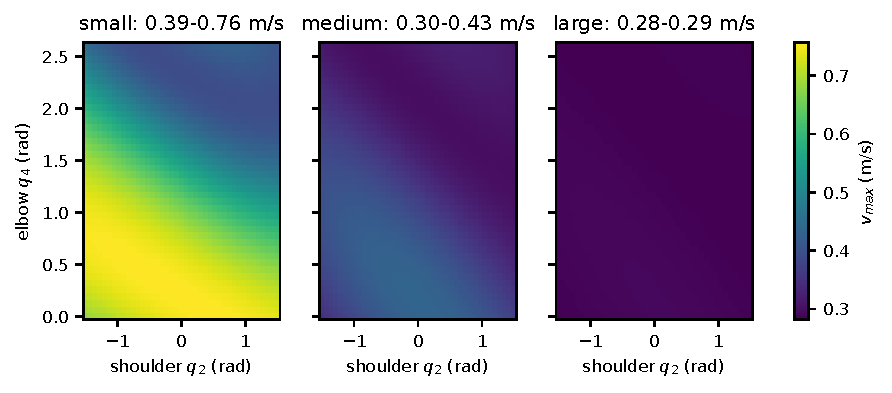
\includegraphics[width=.8\textwidth]{figs/fig5_vmax}
\caption{Permitted hand speed over shoulder and elbow angle.}\label{fig:vmax}\end{figure*}

Fig.~\ref{fig:vmax}: 0.39 to 0.76\,m/s on the 30\,kg servicer, 0.30 to 0.44 on 300\,kg, and 0.28 to
0.29 on 3000\,kg, where the base is so heavy that posture stops mattering. The task's peak hand
speed is 0.063\,m/s, well inside all three. A floating base makes contact gentler, and a light
one more so.

\section{Operator Study}
\todo{Not run. No participant data exists.} Protocol: within-subject, each participant flies one
loop under all 5 schemes $\times$ 2 tasks by gamepad, order shuffled and scheme hidden. After each
trial: a 1--7 predictability rating; after each scheme: NASA-TLX~\cite{hart1988}. Objective
measures are the same as Section~V. Hypothesis: schemes with null-space impedance (3, 5) are rated
more predictable than their counterparts (1, 4). \todo{Fig.~4, statistics, ethics statement.}

\section{Discussion and Conclusion}
The spare joints of a 7-joint arm are worth different things on different spacecraft. For
position-only work inside the level-base envelope, impedance plus RNS is the best of both: quiet base,
repeatable arm. For 6-D
work on a small servicer the operator must be given, or must choose, a point on the trade-off
curve. On a large servicer reaction is negligible and the freedom should go to the operator.
For teleoperation the same trade-off sets the work envelope: the space an operator can be offered
is a choice of how far the base may tilt, and because that tilt is roughly repeatable it can be shown to
the operator before the move rather than discovered during it. Whether a goal is accepted did not depend
on where the hand started: 36 goals on 12 directions, at 0.6, 0.9 and 1.15 of the edge, got the same answer
from rest and after a 0.15\,m detour sideways or upward (72 of 72), even with the base left 0.8$^\circ$ off by
the detour. So one envelope probed from rest along 98 directions can be drawn once: it agreed with a rehearsal
of the move on 271 of 300 goals placed near its edge.

\textbf{Limitations.} One arm, one path, one rest posture; gains tuned by hand on one servicer;
scripted operator only; no flexible appendages, joint friction or sensor noise; initial momentum
zero; safety values are for one body region and a locked-joint worst case.

\bibliographystyle{IEEEtran}
% TODO: check every entry against P2_Literature_Survey.xlsx; these were written from memory.
\begin{thebibliography}{99}
\bibitem{dubowsky1993} S. Dubowsky and E. Papadopoulos, ``The kinematics, dynamics, and control of free-flying and free-floating space robotic systems,'' \emph{IEEE Trans. Robot. Autom.}, vol. 9, no. 5, 1993.
\bibitem{umetani1989} Y. Umetani and K. Yoshida, ``Resolved motion rate control of space manipulators with generalized Jacobian matrix,'' \emph{IEEE Trans. Robot. Autom.}, vol. 5, no. 3, 1989.
\bibitem{nenchev1999} D. N. Nenchev, K. Yoshida, P. Vichitkulsawat, and M. Uchiyama, ``Reaction null-space control of flexible structure mounted manipulator systems,'' \emph{IEEE Trans. Robot. Autom.}, vol. 15, no. 6, 1999.
\bibitem{yoshida2001} K. Yoshida, K. Hashizume, and S. Abiko, ``Zero reaction maneuver: flight validation with ETS-VII space robot and extension to kinematically redundant arm,'' in \emph{Proc. IEEE ICRA}, 2001.
\bibitem{hogan1985} N. Hogan, ``Impedance control: an approach to manipulation,'' \emph{ASME J. Dyn. Syst. Meas. Control}, vol. 107, 1985.
\bibitem{dragan2013} A. D. Dragan, K. C. T. Lee, and S. S. Srinivasa, ``Legibility and predictability of robot motion,'' in \emph{Proc. ACM/IEEE HRI}, 2013.
\bibitem{nakamura1986} Y. Nakamura and H. Hanafusa, ``Inverse kinematic solutions with singularity robustness for robot manipulator control,'' \emph{ASME J. Dyn. Syst. Meas. Control}, vol. 108, 1986.
\bibitem{liegeois1977} A. Li\'egeois, ``Automatic supervisory control of the configuration and behavior of multibody mechanisms,'' \emph{IEEE Trans. Syst. Man Cybern.}, vol. 7, no. 12, 1977.
\bibitem{khatib1995} O. Khatib, ``Inertial properties in robotic manipulation: an object-level framework,'' \emph{Int. J. Robot. Res.}, vol. 14, no. 1, 1995.
\bibitem{iso15066} \emph{Robots and robotic devices -- Collaborative robots}, ISO/TS 15066:2016.
\bibitem{haddadin2012} S. Haddadin \emph{et al.}, ``On making robots understand safety: embedding injury knowledge into control,'' \emph{Int. J. Robot. Res.}, vol. 31, no. 13, 2012.
\bibitem{todorov2012} E. Todorov, T. Erez, and Y. Tassa, ``MuJoCo: a physics engine for model-based control,'' in \emph{Proc. IEEE/RSJ IROS}, 2012.
\bibitem{hart1988} S. G. Hart and L. E. Staveland, ``Development of NASA-TLX: results of empirical and theoretical research,'' in \emph{Human Mental Workload}, 1988.
\end{thebibliography}
\end{document}
